\documentclass[12pt]{article}
 \usepackage[margin=1in]{geometry} 
\usepackage{amsmath,amsthm,amssymb,amsfonts}
\usepackage{graphicx}

 
\newcommand{\N}{\mathbb{N}}
\newcommand{\Z}{\mathbb{Z}}
 
\newenvironment{problem}[2][]{\begin{trivlist}
\item[\hskip \labelsep {\bfseries #1}\hskip \labelsep {\bfseries #2.}]}{\end{trivlist}}

 
\begin{document}
  
\title{Computational Physics Project 1: Pendulum}
\author{Ben Zager, Remy Wang}
\maketitle
 
\section*{The Simple Pendulum}

\noindent
\begin{figure}[ht!]
	\centering
	\begin{minipage}[b]{0.4\textwidth}
	  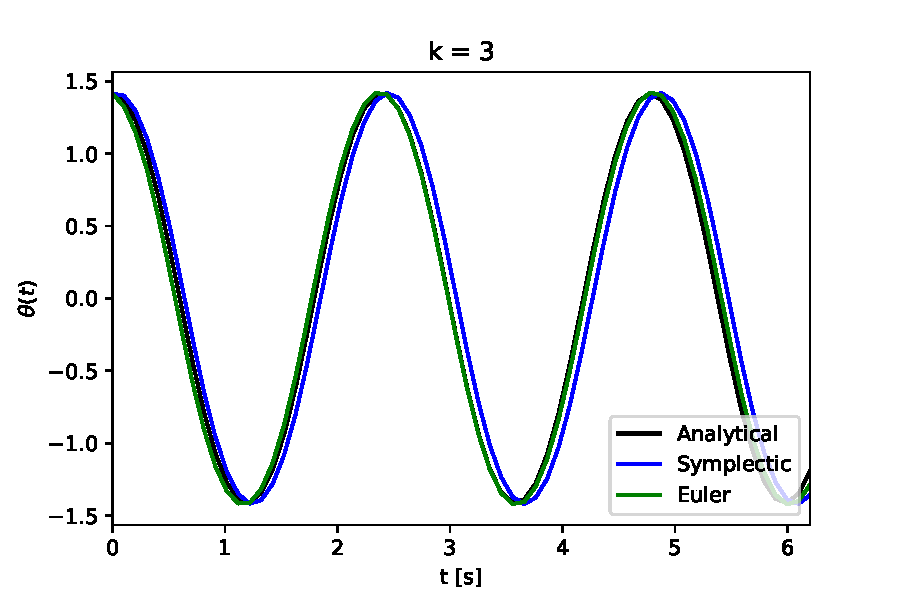
\includegraphics[scale=0.6]{../figures/k3_nonlin.pdf}
		\label{phaseDot}
	\end{minipage}
	\hfill
	\begin{minipage}[b]{0.4\textwidth}
	  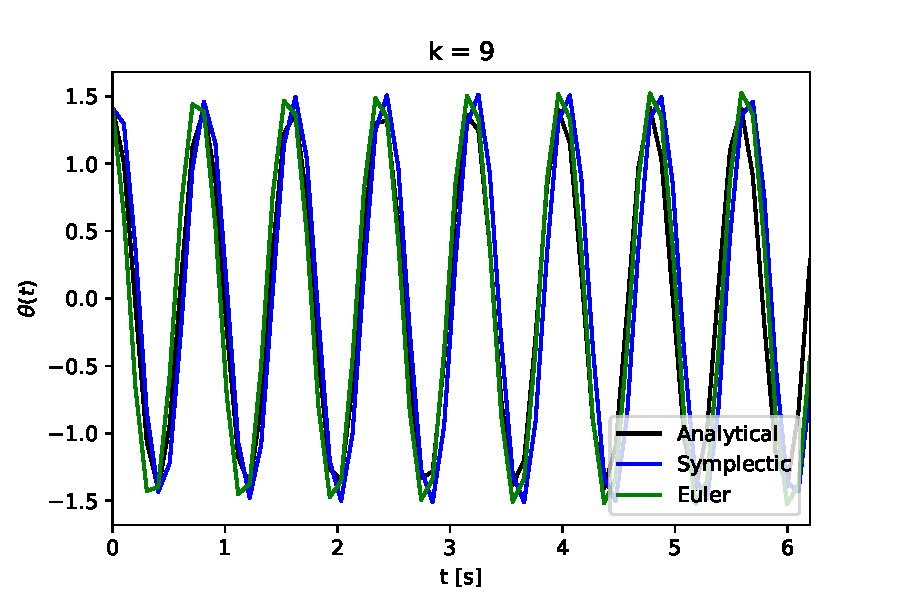
\includegraphics[scale=0.6]{../figures/k9_nonlin.pdf}
		\label{phaseDot2}
	\end{minipage}
	\begin{minipage}[b]{0.4\textwidth}
	  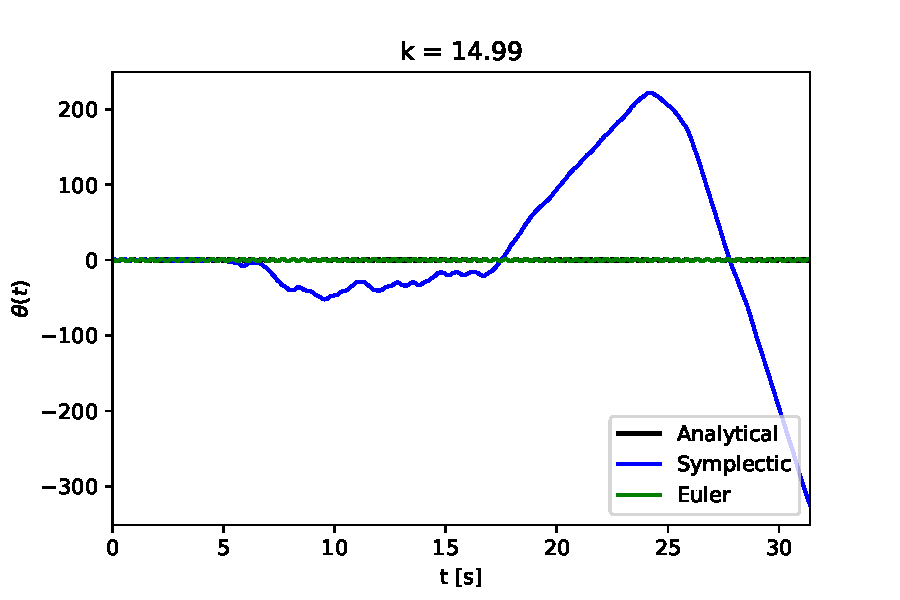
\includegraphics[scale=0.6]{../figures/k15_nonlin.pdf}
		\label{phaseDot2}
	\end{minipage}
	\hfill
	\begin{minipage}[b]{0.4\textwidth}
	  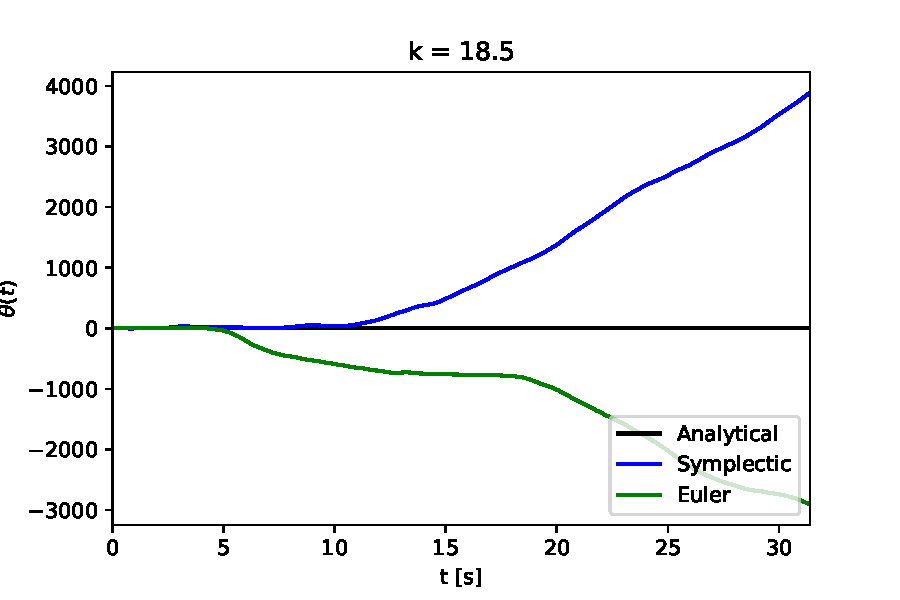
\includegraphics[scale=0.6]{../figures/k17_nonlin.pdf}
		\label{phaseDot2}
	\end{minipage}
	\caption{Trajectory for various $\dot{\theta}$}
\end{figure}

\section*{Route to Chaos}

%%%%%% 1 %%%%%%
\begin{problem}{1}
	\textbf{Phase space of nonlinear pendulum}

	As $\theta_{0}$ approaches $\pi$, the trajectories go from an ellipse to a more "lemon" shape, as seen in figure 1.

	For $\theta_{0} = 0$, varying $\dot{\theta}_{0} \in [0,\pi]$, the phase shows two different behaviors.  For $\dot{\theta}_{0}$ between 0 and approximately $0.6\pi$ the phase space appears similar to the previous one, as seen in figure 2a.  If $\dot{\theta}_{0}$ is greater than that, the motion is no longer periodic, and $\theta$ increases indefinitely, as seen in figure 2b.

\begin{figure}[ht!]
	\centering
	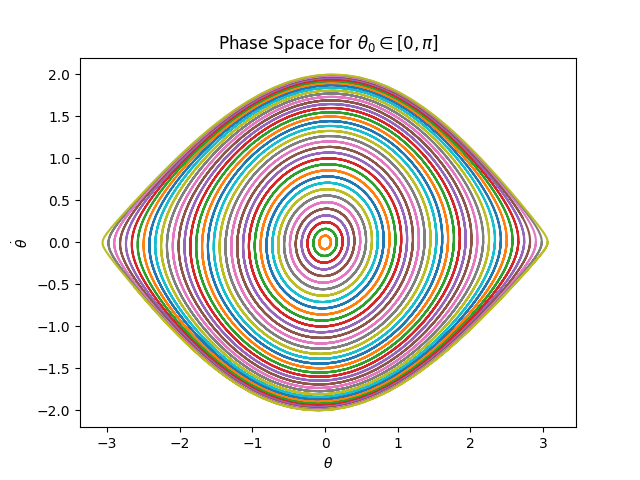
\includegraphics[scale=0.6]{../figures/phaseSpace.png}
	\caption{Plots of trajectory $(\theta,\dot{\theta})$, for many values of $\theta_{0} \in [0,\pi]$}
	3\label{phase}
\end{figure}

\begin{figure}[ht!]
	\centering
	\begin{minipage}[b]{0.4\textwidth}
		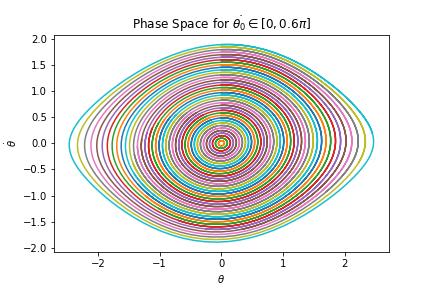
\includegraphics[scale=0.6]{../figures/phaseSpaceDot.png}
		\label{phaseDot}
	\end{minipage}
	\hfill
	\begin{minipage}[b]{0.4\textwidth}
		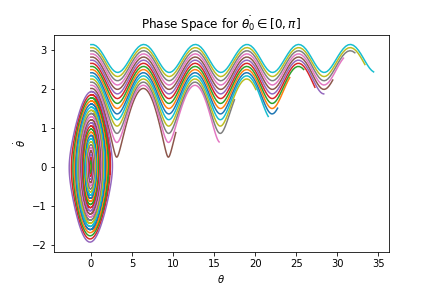
\includegraphics[scale=0.6]{../figures/phaseSpaceDot2.png}
		\label{phaseDot2}
	\end{minipage}
	\caption{Trajectory for various $\dot{\theta}$}
\end{figure}
\end{problem}

%%%%%% 2 %%%%%%
\begin{problem}{2}
	\textbf{Phase space of linear pendulum} \\
	For the linear pendulum, the phase space trajectory remains elliptical for all values of $\theta_{0}$

\begin{figure}[h!]
\centering
  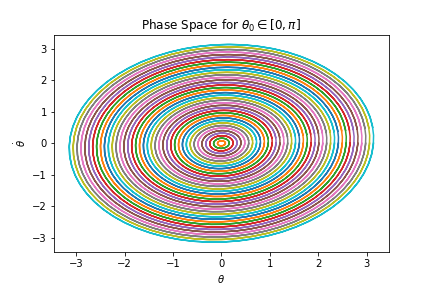
\includegraphics[scale=0.6]{../figures/phaseSpaceLinear.png}
  \caption{Plots of linearized trajectory $(\theta,\dot{\theta})$, for many values of $\theta_{0} \in [0,\pi]$}
  \label{phaseLin}
\end{figure}
\end{problem}

%%%%%% 3 %%%%%%
\begin{problem}{3}
	\textbf{Pendulum with driving force, $\gamma k^{2}cos(\omega t)$} \\
	If a periodic driving force with $\omega = k$ is added, the frequency stays the same, but the ampltude varies periodically, as seen in figure \ref{driving}. 
\begin{figure}[h!]
	\centering
  	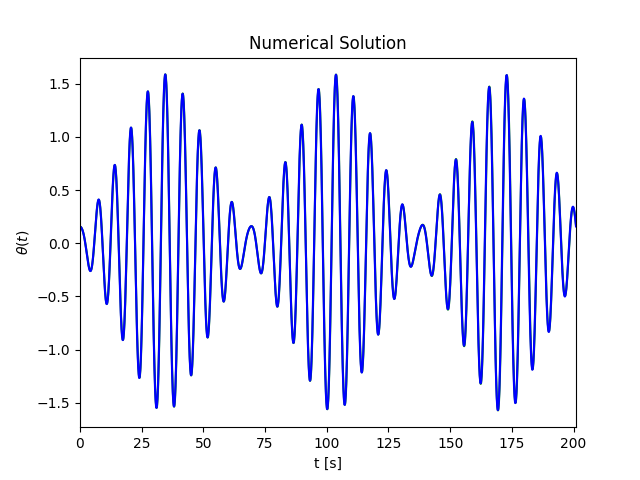
\includegraphics[scale=0.6]{../figures/drivingForce.png}
 	\caption{Solution for driven undamped pendulum}
  	\label{driving}
\end{figure}
\end{problem}

%%%%%% 4 %%%%%%
\begin{problem}{4}
	\textbf{Exploration of driven system} \\
	For fixed $\theta$ and $\dot{\theta}$, how do the real and phase space trajectories vary with $\gamma$.  

	\begin{figure}[ht!]
	\centering
	\begin{minipage}[b]{0.4\textwidth}
		%\includegraphics[scale=0.6]{../figures/.png}
		\label{}
	\end{minipage}
	\hfill
	\begin{minipage}[b]{0.4\textwidth}
		%\includegraphics[scale=0.6]{../figures/.png}
		\label{}
	\end{minipage}
	\caption{}
\end{figure}
\end{problem}

%%%%%% 5 %%%%%%
\begin{problem}{5}
	\textbf{Identifying $(\theta_{0},\gamma)$ for which the motion diverges} \\

	Figure 6 shows the phase plot for $(\theta_{0},\gamma)$ for $\theta_{0} \in [0,\pi]$, and $\gamma \in [0,6]$, after a time interval of $8\pi$ seconds.  The white regions indicate values for which the motion remained periodic. The blue regions indicate values for which the motion diverged.  The darker the color, the greater the value of $\theta$ at the end of the time interval.
\begin{figure}[h!]
	\centering
  	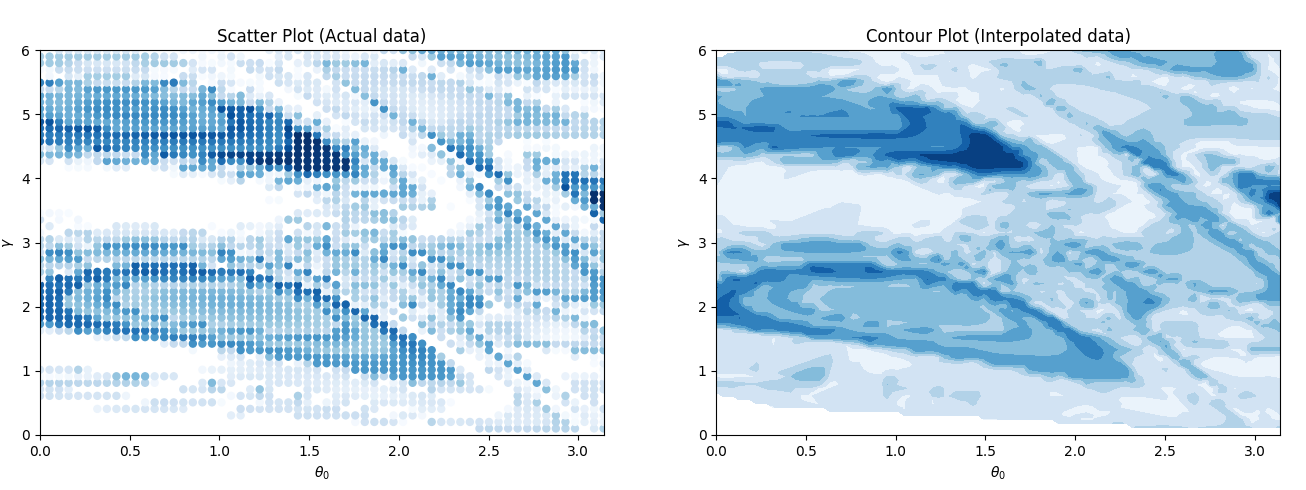
\includegraphics[scale=0.5]{../figures/diverge2.png}
 	\caption{Phase plot for $(\theta_{0},\gamma)$. On the left is the actual data that was calculated, and on the right is an interpolated contour plot.}
  	\label{diverge}
\end{figure}
\end{problem}

%%%%%% 6 %%%%%%
\begin{problem}{6}
	\textbf{Driven pendulum with damping} $\ddot{\theta}+2\beta\dot{\theta}+k^{2}sin\theta=\gamma k^{2}cos(\omega t)$ \\


\end{problem}

%%%%%% 7 %%%%%%
\begin{problem}{7}
	\textbf{Fourier analysis}
\end{problem}

\section*{The Double Pendulum}

\end{document}
